\documentclass[fontsize=11pt]{article}
\usepackage{amsmath}
\usepackage[utf8]{inputenc}
\usepackage[margin=0.75in]{geometry}
\usepackage{graphicx}

\title{CSC110 Project Proposal: Your Anxiety During COVID-19}
\author{Fardin Faruk, Sharon Hsieh, Sinan Li, Jeffery Zhan}
\date{Friday, November 5, 2021}

\begin{document}
    \maketitle

    \section*{Problem Description and Research Question}

    Severe acute respiratory syndrome coronavirus 2 (SARS-CoV-2), commonly known for causing the illness COVID-19, spread wildly after its emergence in late 2019 (Britannica, T. Editors of Encyclopaedia, 2021). Following its discovery, society as we knew it was upended, and countries went into lockdown. Individuals were required to stay home to prevent the spread of the virus, restricting any socializing to very minimal interactions with others. Tested by working from home, unemployment, lack of social connections and many more challenges, many individuals found it challenging to adapt, making them especially vulnerable to mental health complications (World Health Organization, 2021).

    While COVID-19 has proven challenging to combat, Canada has put forth their best efforts to prevent the spread of the virus, becoming one of the top vaccinated countries in the world (Mathieu et al., 2021). Despite social regulations having been eased, many of the psychological effects linger. In fact, mental health has become such a prominent concern due to the pandemic that analysts at The National Institute of Mental Health now describe online therapy as essential (Prout, 2021).

    There is no doubt that the onset of the pandemic affected everyone differently — some found it easy to adjust, some struggled to do so, and many experienced some combination of the two — all for varying reasons. We would like to measure these differences quantitatively. Thus, we decided to research and answer the question: \textbf{what is the relationship between one’s identity and the degree to which COVID-19 has impacted their mental health?}

    Our research will examine various traits that the subjects of the survey have, such as their education level, marital status, gender, and age, then compare their surveyed response to the pandemic alongside their traits and identities to determine a relationship between certain identity groups and the socio-psychological effects COVID-19 has had on them. From the results, we will ascertain which types of people are more susceptible to psychological issues due to the pandemic. We believe that this data can be applied to strengthen mental health resources and allow for more specialized and efficient care.

    \section*{Dataset Description}

    COVIDiSTRESS Global Survey dataset on psychological and behavioural consequences of the COVID-19 outbreak (Yamada et al., 2020) is a survey which was organized by researchers in over 90 universities across the globe, investigating the mental health conditions and personal views surrounding COVID-19. It was conducted during the first major wave of the pandemic, and the responses of approximately 125,000 participants aged 18 and over, ranging across 42 countries, were recorded through this survey. The data is stored in a .csv file with each row containing information about a single person, including their gender, age, occupation status, marital status, and more. The file also includes each participant's responses to a broad range of questions posed on the survey about COVID-19. These questions range from questions about the individual’s support systems to questions about how they obtain information about COVID-19. Most questions were answered through a six-point Likert scale, which will help us to quantify each participant’s responses.

    \begin{figure}
        \centering
        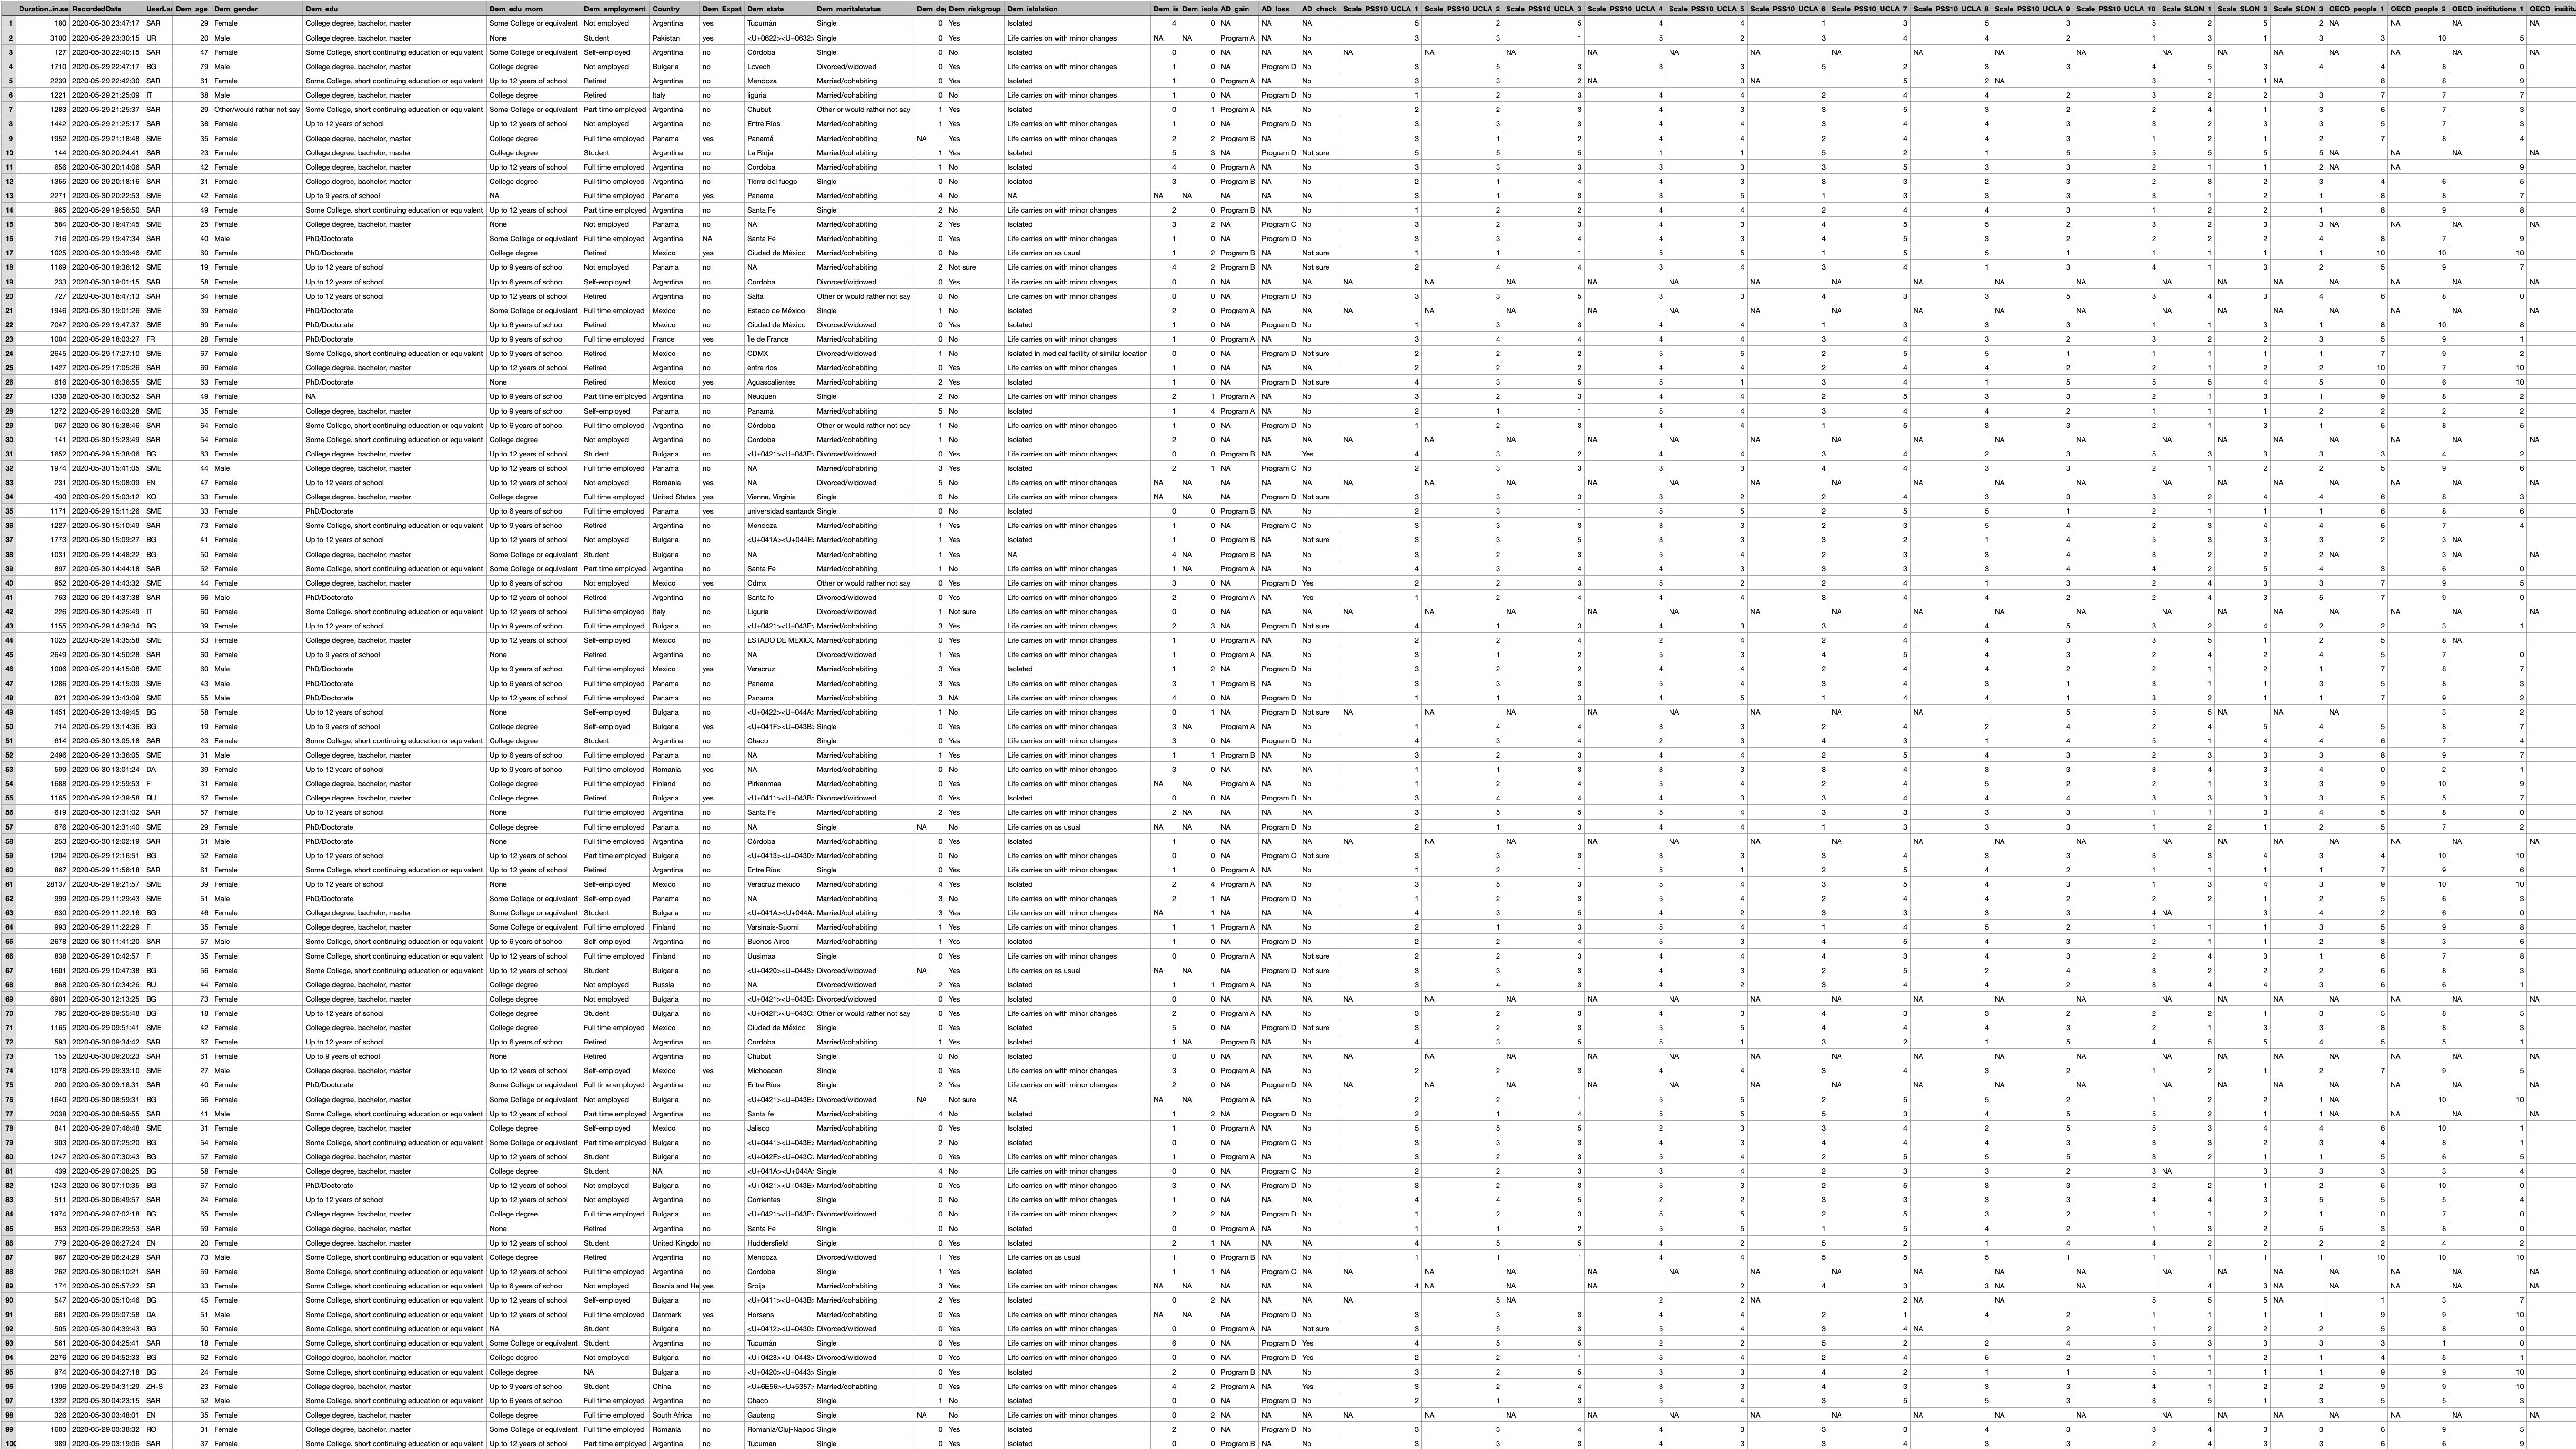
\includegraphics[width=\textwidth]{img/SampleData.png}
        \caption{Sample Data}
        \label{fig:my_label}
    \end{figure}

    \section*{Computational Plan}

    Our computational plan is composed of three stages:

    \begin{itemize}
        \item \textbf{Stage 1:} Read the data from the CSV file containing the test subject’s information and responses

        \begin{itemize}
            \item Create dictionaries categorizing each identity group (e.g. gender, age, etc). The keys are strings representing each identity group (e.g. `Male’, `Female’, or `15to19’, `20to29’, \dots), and the value is an integer that measures an identity group’s average level of anxiety. For now, initialize the values to zero.

            \item Read the data from the CSV file row by row.
        \end{itemize}

        \item \textbf{Stage 2:} Compute the data

        \begin{itemize}
            \item For each row, use the responses to calculate an anxiety score for the entry. Then, go through all dictionaries of every identity group, and add the total score of the entry to the corresponding identity groups. Keep track of the population of each identity group in separate variables.

            \item When all rows have been inputted, calculate the average score for each identity group using the total anxiety scores of the group divided by the population of the identity group.

            \item Find the maximum and minimum anxiety scores from every possible combination of identity groups, label them $s_{\mathrm{max}}$ and $s_{\mathrm{min}}$ respectively. Then calculate their difference, $\Delta s = s_{\mathrm{max}} - s_{\mathrm{min}}$. This is the scale of anxiety levels based on the entire population.
        \end{itemize}

        \item \textbf{Stage 3:} Display the data

        \begin{itemize}
            \item We will first represent the average anxiety level of each category of identity groups using a series of graphs. A user will be able to select which graph they would like to see using a drop-down menu. Attributes such as gender, education, and marital status will be visualized using bar graphs, while age will be displayed using a histogram.

            \item To make the program and experience more engaging for the user, allow the user to select certain identity groups from the menu. The user will be able to compare their mental wellness to not only the overall population, but also to the specific identity group(s) selected, which will be done through separate calculations.

            \begin{itemize}
                \item To calculate the wellbeing of the individual, first calculate the individual’s anxiety score by taking the mean of the anxiety scores of all identity groups relevant to the individual. Label the score $s_{\mathrm{usr}}$. Then, the individual’s relative mental well-being, $r$, can be calculated using the formula $r = \left(1 - \frac{s_{\mathrm{usr}} - s_{\mathrm{min}}}{\Delta s}\right) \times 100 \%$. Display the output ``You are less / more (depending on the percentage) likely to be anxious than $r$ \% of the population." Such ranking can be displayed graphically using a gauge.

                \item From a drop-down list, allow the user to select from all his/her identity groups, which allows the user to see his/her relative ranking in a certain identity group. For example, ``You are less likely than $r_2$ \% of males in terms of being anxious.”, where $r_2$ can be calculated in a similar fashion to $r$, except excluding all other identities in the same group when finding $s_{2,\mathrm{max}}$ and $s_{2,\mathrm{min}}$, essentially narrowing the calculations down to just the selected trait; e.g. if the user selects `Male’, the Female score is ignored in the calculations. Such data can be displayed using a progress bar indicating one’s level of anxiety relative to the rest of the selected population.
            \end{itemize}
        \end{itemize}
    \end{itemize}

    An external library we will be using is \texttt{PyQt5}, a python package providing high-level APIs for the creation of cross-platform programs with a graphical user interface (Riverbank Computing Limited., 2021). Using the signal-slot design pattern, this Python variation of the C++ Qt library allows us to create interactive programs, which can take input from the user in a graphically interactive way -- this fulfils the need of our purpose. Through this project, we will be using the \texttt{QWigit} class provided by this python package, with its subclass \texttt{QPushButton} as interactive buttons, \texttt{QLabel} as text display, \texttt{QLineEdit} as one-line text input, and many more to make the displayed interface organized and engaging. To plot the data, we will be using \texttt{PyQtGraph}, a graphing library designed for PyQt5 (pyqtgraph, 2021). Compared to other mainstreaming plotting libraries, this library provides a fast refresh speed for rapid plot updates, which allows the user of our program to experience low latencies when navigating between the plotted data of different identity groups. This graphing library was designed for scientific purposes, allowing the creation of various kinds of professional-looking graphs. All these properties serve the needs of our program. We will potentially be using the \texttt{pyqtgraph.PlotWidget().plot(x, y)} function to plot the data we want, or use similar functions depending on the type of graphs that need to be created.

    \section*{References}

% NOTE: LaTeX does have a built-in way of generating references automatically,
% but it's a bit tricky to use so we STRONGLY recommend writing your references
% manually, using a standard academic format like APA or MLA.
% (E.g., https://owl.purdue.edu/owl/research_and_citation/apa_style/apa_formatting_and_style_guide/general_format.html)

    \hangindent=0.7cm
    Britannica, T. Editors of Encyclopaedia (2021, August 31). \textit{coronavirus}. \textit{Encyclopedia Britannica}. https://www.britan\\nica.com/science/coronavirus-virus-group

    \hangindent=0.7cm \noindent
    Government of Canada. (2021). https://health-infobase.canada.ca/covid-19/epidemiological-summary- covid-19-cases.html

    \hangindent=0.7cm \noindent
    Mathieu, E., Ritchie, H., Ortiz-Ospina, E., Roser, M., Hasell, J., Appel, C., Giattino, C., \& Rodés-Guirao, L. (2021). A global database of COVID-19 vaccinations. \textit{Nature Human Behaviour}, \textit{5}(7), 947-953. https://doi.org/10.1038/s\\41562-021-01122-8

    \hangindent=0.7cm \noindent
    Prout, T. (2021, July 8). The importance of mental health during a pandemic. \textit{National University}. Retrieved November 3, 2021, from https://www.nu.edu/resources/the-importance-of-mental-health-during-a-pandemic/

    \hangindent=0.7cm \noindent
    pyqtgraph. (2021). \textit{PyQtGraph} (version 0.12.3) [Computer software]. https://www.pyqtgraph.org/

    \hangindent=0.7cm \noindent
    Riverbank Computing Limited. (2021). \textit{PyQt5} (Version 5.15.6) [Computer software]. https://pypi.org/project/PyQt5/

    \hangindent=0.7cm \noindent
    World Health Organization. (2021). \textit{\#HealthyAtHome - Mental health}. https://www.who.int/campaigns/connecting-the-world-to-combat-coronavirus/healthyathome/healthyathome---mental-health

    \hangindent=0.7cm \noindent
    Yamada, Y., Ćepulić, D.-B., Coll-Martín, T., Debove, S., Gautreau, G., Han, H., Rasmussen, J., Tran, T. P., Travaglino, G. A., Blackburn, A. M., Boullu, L., Bujić, M., Byrne, G., Caniëls, M. C. J., Flis, I., Kowal, M., Rachev, N. R., Reynoso-Alcántara, V., Zerhouni, O. … Consortium, C. O. G. S. (2021). COVIDiSTRESS Global Survey dataset on psychological and behavioural consequences of the COVID-19 outbreak. \textit{Scientific Data}, \textit{8}(1), 3. https://doi.org/10.1038/ s41597-020-00784-9

\end{document}
